%-------------------------------------------------------------------------------
% Laboratório de Redes - 09
% Data do experimento: 23/02/2016
%-------------------------------------------------------------------------------
\documentclass[12pt,a4paper]{article}%

% Tabelas
\usepackage{multirow}
\usepackage{booktabs}
\newcommand{\tabitem}{~~\llap{\textbullet}~~}
\usepackage{longtable}

% Símbolos Matemáticos
\usepackage{amsmath}
\usepackage{amsfonts}
\usepackage{amssymb}
\usepackage{bm}
\usepackage{commath}
\usepackage{steinmetz}
\usepackage{mathrsfs}

% Figuras
\usepackage{graphicx}
\usepackage{wrapfig}
\usepackage{float}
\usepackage{subfig}
\graphicspath{ {img/} }

% Língua e acentos
\usepackage[brazil]{babel}
\usepackage[utf8]{inputenc}
\usepackage[T1]{fontenc}

% Espaçamento
\usepackage[top=3cm, bottom=2cm, left=2cm, right=2cm]{geometry}
\usepackage{indentfirst}

% Pagina em branco
\usepackage{afterpage}
\newcommand \blankpage{
	\null
	\thispagestyle{empty}
	\addtocounter{page}{-1}
	\newpage}

% Lista de códigos
\usepackage{caption}
\usepackage{listings}                  
\usepackage{color}

\definecolor{mygreen}{rgb}{0,0.6,0}
\definecolor{mygray}{rgb}{0.5,0.5,0.5}
\definecolor{mymauve}{rgb}{0.58,0,0.82}

\lstset{ %
    backgroundcolor=\color{white},
    basicstyle=\footnotesize,
    breaklines=true,                 % sets automatic line breaking
    captionpos=t,                    % sets the caption-position to bottom
    commentstyle=\color{mygreen},    % comment style
    extendedchars=true,
    frame=single,	                 % adds a frame around the code
    keepspaces=true,                 % useful for keeping indentation of code
    keywordstyle=\color{blue},       % keyword style
    language=matlab,                 % the language of the code
    otherkeywords={...},           	 % if you want to add more keywords
    numbers=left,                    % where to put the line-numbers
    numbersep=5pt,                   % how far the numbers are from the code
    %numberstyle=\tiny\color{mygray}, % the style that is used for the line-numbers
    rulecolor=\color{black},
    stepnumber=1,                    % the step between two line-numbers.
    stringstyle=\color{mymauve},     % string literal style
    tabsize=2,	                    % sets default tabsize to 2 spaces
    title=\lstname                   % show the filename of files included
}
% Enumerate
\usepackage{enumitem}

% Diagramas
\usepackage{tikz}
\usetikzlibrary{positioning}

% Bibliografia
\usepackage[numbers]{natbib}
%-------------------------------------------------------------------------------

\begin{document}
\begin{titlepage}
\begin{center}
\begin{figure}[h]
\includegraphics[scale=0.76]{Imagens/topdotitulo.png}
\end{figure}
\rule{\columnwidth}{1.5mm}
\

\large David Maykon Krepsky Silva\\
\large Havena Louise Pavão\\

\vspace{4cm}
{\bf \Large Oscilador LC}
\vspace{3.5cm}

\begin{flushright}
Data de realização do experimento:\\
16 de junho de 2016\\
Série/Turma:\\
1000/1011\\
Prof. Me. Jaime Laelson Jacob 
\end{flushright}

\vspace{3.2cm}
\today

\rule{\columnwidth}{1.3mm}
\end{center}
\end{titlepage}
\input{sumario}
\newpage
\begin{abstract}
\addcontentsline{toc}{section}{Resumo}


Neste trabalho foi realizado o estudo teórico de filtros passivos compostos indutores e capacitores (filtros LC) de forma a analisar a resposta em frequência para filtros FPB, FPA, FPF e FPF em cascata. A metodologia utilizada consiste em realizar o projeto do filtro normalizado, transformar para o tipo de filtro requerido e simular o circuito no software Orcad.
Durante o laboratório foi possível observar as diferentes respostas em frequência para cada tipo de filtro estudado.Também foi visualizado a melhora no fator Q de filtros em cascata em relação a um filtro FPF comum.
\end{abstract}
\newpage
\blankpage
\newpage

\section{Introdução}
Os conversores cc/cc do tipo buck tem uma elevada eficiência (maior que70\%). Neste tipo de circuito, um elemento funciona como chave, o ideal é que ele opere ora em corte (quando então a corrente é quase nula), ora em saturação (quando a tensão entre os terminais é quase nula) assim ligando e desligando rapidamente, de forma a manter uma tensão de saída estabilizada, o produto V.I que corresponde à potência dissipada pelo transistor em condução permanece sempre baixo aumentando a eficiência da fonte. Evidentemente, na prática a potência no elemento série não é totalmente nula, mas através de técnicas de circuito adequada e a escolha de componentes melhores, esta potência pode ser reduzida a valores relativamente baixos em comparação com a dissipada nas fontes lineares, assim tendo uma maior eficiência, menor tamanho e maior leveza, entretanto, são complexos e mais caros, e o chaveamento da corrente pode causar problemas de ruído se não forem cuidadosamente suprimidos, também é importante destacar, entretanto, que a ondulação de saída em fontes chaveadas é muito maior em relação às fontes lineares (quase uma ordem de grandeza). Outro fator importante é que a eficiência de tais fontes varia de acordo com a potência de saída, tendo uma menor eficácia na conversão de energia para uma carga maior do que a projetada.
\newpage
\section{Revisão da Teoria}

\subsection{Conversor \textit{Boost}}

O principio de funcionamento do conversor \textit{Boost} é que um indutor cria e destrói um campo magnético para resistir a mudanças bruscas de corrente. Isso permite que a tensão de saída do circuito seja maior que a tensão de entrada. Neste trabalho será analisado somente o caso em que o indutor nunca é descarregado por completo (modo contínuo).

A figura \ref{fig:boost2} mostra um esquemático do conversor \textit{Boost}. O circuito opera em dois estados, que dependem da chave T. Estes estados são descritos abaixo.

\begin{itemize}
    \item \textbf{Chave T Fechada:} Quando a chave T está fechada (\ref{fig:tclosed}), a corrente $I_L$ flui através do indutor L, no sentido horário. Isso faz com que o indutor armazene energia na forma de campo magnético. Enquanto o interruptor carrega, uma tensão $V_l$ aparece sobre o mesmo, tendo como lado positivo o lado esquerdo.
    
    \item \textbf{Chave T Aberta:} Ao abrir a chave, a corrente $I_L$ que passava no indutor se manterá (não há variação de corrente instantânea no indutor), porém a tensão em cima do mesmo será diferente, dado que a impedância vista pelo indutor mudou. Para manter a corrente, o campo magnético que havia sido criado previamente, será agora destruído. Isso fará com que a polaridade da tensão em cima do indutor ($V_L$) mude de sentido. Do ponto de vista da carga, agora são duas fontes de tensão em série, como indicado na figura \ref{fig:opened}.
\end{itemize}


\begin{figure}[H]
    \centering
    \caption{Esquemático do conversor \textit{Boost}.}
    \includegraphics[scale = 0.5]{boost2}
    \label{fig:boost2}
    
    \small Fonte: Autoria própria.
\end{figure}

Vale notar que, para que o conversor opere no modo contínuo, a frequência de chaveamento deve ser alta o suficiente para manter uma carga mínima no indutor.

Um característica importante do conversor \textit{Boost} é que a corrente de entrada é constante, ou seja, há pouco ruído indo para a fonte de alimentação.

\subsubsection{Ganho estático}

    Para os cálculos do ganho de tensão no conversor \textit{Boost}, vamos considerar os componentes ideais, o circuito no regime estático de operação e que a corrente no indutor nunca chega a zero (modo contínuo).
    
    Quando a chave está fechada (figura \ref{fig:tclosed}), aparece uma tensão $V_i$ em cima do indutor, a qual causa uma corrente $I_L$ através do indutor durante um período de tempo $\tau$. A corrente e a tensão no indutor estão relacionadas pela equação geral do indutor (\ref{equ:Vl}).
    
    \begin{equation}
        V_L = L\frac{\Delta I_L}{\Delta t}
        \label{equ:Vl}
    \end{equation}

    Ao final do período $\tau$, a corrente $I_L$ é
    
    \begin{equation}
        \Delta I_{L_{On}}=\frac{1}{L}\int_0^{D T}V_i d t=\frac{D T}{L} V_i.
        \label{equ:ilon}
    \end{equation}
    
    Onde D é a razão cíclica (fração do período T no qual a chave T fica fechada).

    \begin{figure}[H]
        \centering
        \caption{Conversor \textit{Boost} com a chave T fechada.}
        \includegraphics[scale = 0.5]{tclosed}
        \label{fig:tclosed}
        
        \small Fonte: Autoria própria.
    \end{figure}

    Ao abrir a chave (figura \ref{fig:opened}), a corrente que passa através do diodo fluirá através da carga. Porém, conforme a energia no indutor é transferida para a carga, a tensão no indutor diminui. Assim, a tensão $V_L$ será

    \[
        V_L = V_i-V_o = L\frac{dI_L}{dt}.
    \]

    Então, a variação de $I_L$ se da por

    
    \begin{equation}
        \Delta I_{L_{Off}}=\int_{DT}^{T}\frac{\left(V_i-V_o\right) dt}{L}=\frac{\left(V_i-V_o\right) \left(1-D\right) T}{L}.
        \label{equ:iloff}
    \end{equation}
    

\begin{figure}[H]
    \centering
    \caption{Conversor \textit{Boost} com a chave T aberta.}
    \includegraphics[scale = 0.5]{topened}
    \label{fig:opened}
    
    \small Fonte: Autoria própria.
\end{figure}

    Para que o indutor não sature, é necessário que a energia armazena durante o período de carregamento seja liberada durante o período de descarregamento do indutor. Ou seja

    
    \begin{equation}
        \Delta I_{L_{On}} + \Delta I_{L_{Off}}=0.
        \label{equ:dilzero}
    \end{equation}
    
    
    Substituindo \ref{equ:ilon} e \ref{equ:iloff} em \ref{equ:dilzero}, temos que
    
    \[
        \Delta I_{L_{On}} + \Delta I_{L_{Off}}=\frac{V_i D T}{L}+\frac{\left(V_i-V_o\right)\left(1-D\right)T}{L}=0.
    \]

    A qual pode ser reescrita como
    
    \begin{equation}
        \frac{V_o}{V_i}=\frac{1}{1-D}.
        \label{equ:ganho}
    \end{equation}
    
    Esta é a equação do ganho estático para o conversor \textit{Boost} em modo contínuo. Observe que a tensão de saída será sempre maior ou igual a tensão de entrada e que, teoricamente, a tensão de saída sobe até o infinito conforme D se aproxima de 1.
    
    \subsection{Conversor \textit{Flyback}}
    A análise do conversor \textit{flyback} da figura \ref{fig:flyback2} e dada nas etapas a seguir.
    
    \begin{figure}[H]
      \centering
      \caption{Esquemático do conversor \textit{Flyback}.}
      \includegraphics[scale = 1]{flyback2}
      \label{fig:flyback2}
      
      \small Fonte: INEP \cite{INEP}.
    \end{figure}
    
    \begin{enumerate}
      \item \textbf{Etapa $\mathbf{(0, DT_s)}$:}  S está conduzindo. A fonte $V_i$ fornece energia para a magnetização do enrolamento primário do transformador. O diodo D está reversamente polarizado.
      
      \item \textbf{Etapa $\mathbf{(DT_s, (1-D)T_s)}$:}  S está bloqueado. A energia armazenada no transformador é levada para a saída através do diodo D. A forma de onda da tensão no primário do transformador é mostrada na figura \ref{fig:flyback3}.
      
      \begin{figure}[H]
        \centering
        \caption{Tensão no primário.}
        \includegraphics[scale = 0.7]{flyback3}
        \label{fig:flyback3}
        
        \small Fonte: INEP \cite{INEP}.
      \end{figure}
    \end{enumerate}
    
    A relação entre a tensão de saída e a tensão de entrada, utilizando uma aproximação de circuito ideal, é dada pela equação \ref{equ:flyback}.
    
    \begin{equation}
    \label{equ:flyback}
    \frac{V_o}{V_i} = \frac{D}{1-D}
    \end{equation}
    
    Essa equação não leva em consideração o ganho devido ao transformador, que deve ser considerado nos cálculos.
    
    A figura \ref{fig:flyback4} mostra as principais formas de onda do conversor \textit{flyback}.

    \begin{figure}[H]
      \centering
      \caption{Formas de onda no conversor \textit{flyback}.}
      \includegraphics[scale = 0.5]{flyback4}
      \label{fig:flyback4}
      
      \small Fonte: INEP \cite{INEP}.
    \end{figure}
\newpage
\section{Metodologia Experimental}

\subsection{Materiais}
O material utilizado foi:
\begin{itemize}
\item Computador.
\item Software Orcad.
\end{itemize}

\subsection{Métodos}

\subsubsection{Redes Adaptadoras de Banda Estreita: 2 e 3 elementos (L, T e $\pi$)}

1- A partir do circuito da figura \ref{fig:redeL}, projetar uma rede adaptadora de impedância com 2 elementos (rede L) tal que $Z_{in} = 50 \ \Omega$ em $\omega_0 = 4300 krad/s$; com impedância de saída $Z_{out} = 1k\Omega$. Admita que a rede tenha também a função de bloquear a eventual componente DC a fonte.

\begin{figure}[H]
    \centering
    \caption{Rede L.}
    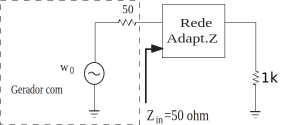
\includegraphics[scale=1]{Imagens/redeL.pdf}
    \label{fig:redeL}
    
    \small Fonte: Me. Jaime Laelson Jacob, 2016.
\end{figure}

\begin{enumerate}[label=\alph*]
    \item Montar o circuito com a rede adaptadora projetada;
    
    \item Injetar um sinal senoidal de frequência $\omega_0$ e
    amplitude da ordem de centenas de milivolts de pico na entrada do circuito montado.
    
    \item Observar a forma de onda da entrada, sobre a carga à saída e sobre a carga resistiva à saída. Anotar as formas de onda.
    
    \item Variar a frequência do sinal senoidal até obter o perfeito casamento de impedância entre fonte e carga. Anotar esta frequência.
    
    \item Obter o índice de mérito do circuito completo ($Q_{Load}$). Calcular este paramento e comparar com o medido. Obter a banda de passagem da rede adotando um dos critérios para adaptação de impedância, sintetizados nas equações (6) e (7).
   \end{enumerate} 

2- Reprojetar a rede adaptadora utilizando 3 elementos (rede T ou $\pi$). Admita agora que não há restrição para o bloqueio de eventuais componentes
DC entre fonte e carga.
\begin{enumerate}[label=\alph*]
    \item Variar a frequência do sinal senoidal até obter o perfeito casamento de impedância entre fonte e carga. Anotar esta frequência.
    
    \item  Obter, através de um procedimento experimental, o novo índice de mérito carregado para a rede de 3 elementos. Comparar com o valor teórico do projeto.
    
    \item Qual a banda de passagem para esta topologia. Adote o mesmo critério utilizado anteriormente.
\end{enumerate}


\subsubsection{Rede Adaptadora de Banda Larga (WBand)}

A partir do problema de adaptação de impedância mostrado na figura 2, calcular e implementar uma rede de banda larga de 2 seções L de tal forma a maximizar a banda de passagem. Nesta condição, calcular o índice de qualidade carregado do circuito. Como frequência central de projeto, adote a mesma do item anterior.

Passos experimentais:
\begin{enumerate}[label=\alph*]
    \item Montar o circuito com a rede adaptadora WBand projetada.
    
    \item  Obter a BW da rede adotando o mesmo critério utilizado anteriormente na obtenção da BW da rede de banda estreita. Comparar o incremento na BW com relação ao caso anterior.
    
    \item Medir o $Q_{rede}$ WBand e comparar com o valor teórico.
\end{enumerate}


\newpage
\section{Resultados}

\subsection{4-PAM com codificação binária}

Na figura \ref{fig:sinais1}, são mostrados os sinais do sistema PAM com codificação binária. Como pode-se notar na legenda observa-se os pontos onde ocorreu a leitura de sinal. Como nota-se quando comprara-se o sinal transmitido ao recebido, percebe-se um atraso de aproximadamente 6 bits.

\begin{figure}[H]
    \centering
    \includegraphics[scale=0.4]{sinalbin}
    \caption{Sinais obtidos.}
    \label{fig:sinais1}
\end{figure}

Quanto ao desempenho do sistema, a tabela \ref{tab:3} mostra a taxa de erro de bit e a probabilidade de erro em função da razão energia de bit e potência do ruído, sendo que a figura \ref{fig:bin} mostra a representação gráfica da BERx$\frac{Eb}{No}$.

\begin{small}
    \begin{table}[H]
        \begin{center}
            \caption{Tabela BER x Eb/No}
            \begin{tabular}{c|c|c}
                \hline
                $\frac{Eb}{No}$ [dB] & BER & $P_b$ \\
                \hline
                $\infty$ & 0 & 0 \\
                \hline
                10 & 0.0031  & $2.4 \times 10^{-3} $ \\
                \hline
                8 & $1.28 \times 10^{-3}$ & 0.0123 \\
                \hline
                6 & 0.0396 &  0.0372 \\
                \hline
                4 & 0.077 &  0.0782 \\
                \hline
                2 & 0.1311 & 0.1301 \\
                \hline
                0 & 0.1821 & 0.1855 \\
                \hline
            \end{tabular}
            \label{tab:3}
        \end{center}
    \end{table}
\end{small}

\begin{figure}[H]
    \centering
    \includegraphics[scale=0.4]{bin}
    \caption{BER com código binário.}
    \label{fig:bin}
\end{figure}



\subsection{4-PAM com codificação Gray}

Na figura \ref{fig:sinais2}, são mostrados os sinais do sistema PAM com codificação gray. Como pode-se notar na legenda observa-se os pontos onde ocorreu a leitura de sinal. Como nota-se quando comprara-se o sinal transmitido ao recebido, percebe-se um atraso de aproximadamente 6 bits.

\begin{figure}[H]
    \centering
    \includegraphics[scale=0.4]{sinalgray}
    \caption{Sinais obtidos.}
    \label{fig:sinais2}
\end{figure}

Quanto ao desempenho do sistema, a tabela \ref{tab:4} mostra a taxa de erro de bit e a probabilidade de erro em função da razão energia de bit e potência do ruído, sendo que a figura \ref{fig:gray} mostra a representação gráfica da BERx$\frac{Eb}{No}$.

\begin{small}
    \begin{table}[H]
        \begin{center}
            \caption{Tabela BER x Eb/No}
            \begin{tabular}{c|c|c}
                \hline
                $\frac{Eb}{No}$ [dB] & BER & $P_b$ \\
                \hline
                $\infty$ & 0 & 0 \\
                \hline
                10 & 0.0019 & $1.8 \times 10^{-3} $ \\
                \hline
                8 & $8.6 \times 10^{-3}$ & 0.0092 \\
                \hline
                6 & 0.0274 &  0.0279 \\
                \hline
                4 & 0.0595 & 0.0586 \\
                \hline
                2 & 0.0954 & 0.0976 \\
                \hline
                0 & 0.1463 & 0.1392 \\
                \hline
            \end{tabular}
            \label{tab:4}
        \end{center}
    \end{table}
\end{small}

\begin{figure}[H]
    \centering
    \includegraphics[scale=0.4]{gray}
    \caption{BER com código Gray.}
    \label{fig:gray}
\end{figure}


Para finalizar, a figura \ref{fig:bxg} mostra o gráfico de desempenho para as duas codificações, onde nota-se claramente a vantagem da codificação gray em relação a codificação binária.

\begin{figure}[H]
    \centering
    \includegraphics[scale=0.4]{bxg}
    \caption{Exemplo de figura}
    \label{fig:bxg}
\end{figure}
\newpage
\section{Discussão e Conclusão}
As simulações tiveram resultados condizentes com a teoria, comprovando na prática, diversos circuitos relacionados com esse relatório sobre modulações ASK, PSK e FSK. É super interessante observar essas modulações na prática para ter convicção e compreensão de seus funcionamentos. As primeiras imagens de cada item na parte experimental provam todos esses funcionamentos.
Sobre a BER, observa-se um valor bastante próximo entre teoria e prática, gerando maior confiabilidade nos sistemas na hora de implementação dentro de um circuito, porém na última imagem (41) é onde encontra-se o maior resultado, onde compara-se todas as 3 modulações e verifica-se que a modulação PSK possui uma atenuação muito menor se comparado com os outros tipos de modulação, não que as outras sejam ruins, porém a PSK é um método que consegue garantir garantia do sinal próximo de íntegro de uma transmissão no meio de telecomunicações.
\newpage

\nocite{*}
\bibliography{config}{}
\bibliographystyle{ieeetr}
\end{document}